\documentclass[a4paper]{book}
\usepackage{graphics}
\pagenumbering{roman}

%------------------------------------------------------------------------------
\newcommand{\stardoccategory}  {Starlink User Note}
\newcommand{\stardocinitials}  {SUN}
\newcommand{\stardocnumber}    {206.1}
\newcommand{\stardocauthors}   {P N Daly}
\newcommand{\stardoccoauthor}  {K Krisciunas}
\newcommand{\stardoccocoauthor} {A Bridger}
\newcommand{\stardocaddress}   {pnd$@$jach.hawaii.edu, kevin$@$jach.hawaii.edu, ab$@$jach.hawaii.edu}
\newcommand{\stardocdate}      {19 August 1996}
\newcommand{\stardoctitle}     {Portable--CGS3DR \\
                                CGS3 Data Reduction}
\newcommand{\stardocversion}   {Version V1.0-0}
\newcommand{\stardocmanual}    {Users' Guide}
%------------------------------------------------------------------------------
\newcommand{\radec}     {$[\alpha,\delta\,]$}
\newcommand{\hadec}     {$[h,\delta\,]$}
\newcommand{\azel}      {$[Az,El\,]$}
\newcommand{\gal}       {$[l^{I\!I},b^{I\!I}]$}
\newcommand{\xy}        {$[x,y\,]$}
\newcommand{\xyz}       {$[x,y,z\,]$}
\newcommand{\xyzd}      {$[\dot{x},\dot{y},\dot{z}\,]$}
\newcommand{\xyzxyzd}   {$[x,y,z,\dot{x},\dot{y},\dot{z}\,]$}
\newcommand{\arcsec}    {$\hspace{-0.05em}\raisebox{-0.5ex}
                        {$^{'\hspace{-0.1em}'}$}
                        \hspace{-0.7em}.\hspace{-0.05em}$}
\newcommand{\tsec}      {\mbox{$^{\rm s}\!\!.$}}
\newcommand{\hms}[4]    {$#1^{\rm h}\,#2^{\rm m}\,#3\tsec#4$}
\newcommand{\dms}[4]    {$#1^{\circ}\,#2\raisebox{-0.5ex}{$^{'}$}\,#3\arcsec#4$}
%------------------------------------------------------------------------------
\newcommand{\stardocname}{\stardocinitials /\stardocnumber}
\markright{\stardocname}
\setlength{\textwidth}{160mm}
\setlength{\textheight}{230mm}
\setlength{\topmargin}{-2mm}
\setlength{\oddsidemargin}{0mm}
\setlength{\evensidemargin}{0mm}
\setlength{\parindent}{0mm}
\setlength{\parskip}{\medskipamount}
\setlength{\unitlength}{1mm}
\renewcommand{\_}{{\tt\char'137}}
\voffset = -1.0cm
%------------------------------------------------------------------------------
% Add any \newcommand or \newenvironment commands here
\renewcommand{\thepage}{\roman{page}}
%  Define length variables.
\newlength{\sstbannerlength}
\newlength{\sstcaptionlength}
%  Define a \tt font of the required size.
\font\ssttt=cmtt10 scaled 1095
%  Define a command to produce a routine header, including its name,
%  a purpose description and the rest of the routine's documentation.
\newcommand{\sstroutine}[3]{
   \goodbreak
   \rule{\textwidth}{0.5mm}
   \vspace{-7ex}
   \newline
   \settowidth{\sstbannerlength}{{\Large {\bf #1}}}
   \setlength{\sstcaptionlength}{\textwidth}
   \addtolength{\sstbannerlength}{0.5em}
   \addtolength{\sstcaptionlength}{-2.0\sstbannerlength}
   \addtolength{\sstcaptionlength}{-4.45pt}
   \parbox[t]{\sstbannerlength}{\flushleft{\Large {\bf #1}}}
   \parbox[t]{\sstcaptionlength}{\center{\Large #2}}
   \parbox[t]{\sstbannerlength}{\flushright{\Large {\bf #1}}}
   \begin{description}
      #3
   \end{description}
}
%  Format the description section.
\newcommand{\sstdescription}[1]{\item[Description:] #1}
%  Format the usage section.
\newcommand{\sstusage}[1]{\item[Usage:] \mbox{} \\[1.3ex] {\ssttt #1}}
%  Format the invocation section.
\newcommand{\sstinvocation}[1]{\item[Invocation:]\hspace{0.4em}{\tt #1}}
%  Format the arguments section.
\newcommand{\sstarguments}[1]{
   \item[Arguments:] \mbox{} \\
   \vspace{-3.5ex}
   \begin{description}
      #1
   \end{description}
}
%  Format the returned value section (for a function).
\newcommand{\sstreturnedvalue}[1]{
   \item[Returned Value:] \mbox{} \\
   \vspace{-3.5ex}
   \begin{description}
      #1
   \end{description}
}
%  Format the parameters section (for an application).
\newcommand{\sstparameters}[1]{
   \item[Parameters:] \mbox{} \\
   \vspace{-3.5ex}
   \begin{description}
      #1
   \end{description}
}
%  Format the examples section.
\newcommand{\sstexamples}[1]{
   \item[Examples:] \mbox{} \\
   \vspace{-3.5ex}
   \begin{description}
      #1
   \end{description}
}
%  Define the format of a subsection in a normal section.
\newcommand{\sstsubsection}[1]{\item[{#1}] \mbox{} \\}
%  Define the format of a subsection in the examples section.
\newcommand{\sstexamplesubsection}[1]{\item[{\ssttt #1}] \mbox{} \\}
%  Format the notes section.
\newcommand{\sstnotes}[1]{\item[Notes:] \mbox{} \\[1.3ex] #1}
%  Provide a general-purpose format for additional (DIY) sections.
\newcommand{\sstdiytopic}[2]{\item[{\hspace{-0.35em}#1\hspace{-0.35em}:}] \mbox{} \\[1.3ex] #2}
%  Format the implementation status section.
\newcommand{\sstimplementationstatus}[1]{
   \item[{Implementation Status:}] \mbox{} \\[1.3ex] #1}
%  Format the bugs section.
\newcommand{\sstbugs}[1]{\item[Bugs:] #1}
%  Format a list of items while in paragraph mode.
\newcommand{\sstitemlist}[1]{
  \mbox{} \\
  \vspace{-3.5ex}
  \begin{itemize}
     #1
  \end{itemize}
}
%  Define the format of an item.
\newcommand{\sstitem}{\item}
%  Define cross and tick, footnote symbols
\newcommand{\cross}{$\times$}
\newcommand{\tick}{$\surd$}
\renewcommand{\thefootnote}{\fnsymbol{footnote}}

%End of LAYOUT.TEX layout definitions.
%------------------------------------------------------------------------------

\begin{document}
\thispagestyle{empty}
CCLRC / {\sc Rutherford Appleton Laboratory} \hfill {\bf \stardocname}\\
{\large Particle Physics \& Astronomy Research Council}\\
{\large Starlink Project\\}
{\large \stardoccategory\ \stardocnumber}
\begin{flushright}
\stardocauthors\footnote[2]{{\em Present Address:}
 {\sf Joint Astronomy Centre, 660 N. A'oh\={o}k\={u} Place, University Park,
  Hilo HI 96720, USA.}},\stardoccoauthor\footnote[3]{{\em Present Address:}
 {\sf Joint Astronomy Centre, 660 N. A'oh\={o}k\={u} Place, University Park,
  Hilo HI 96720, USA.}},\stardoccocoauthor\footnote[4]{{\em Present Address:}
 {\sf Joint Astronomy Centre, 660 N. A'oh\={o}k\={u} Place, University Park,
  Hilo HI 96720, USA.}} \\
{\em \stardocaddress} \\
\stardocdate
\end{flushright}
\vspace{-4mm}
\rule{\textwidth}{0.5mm}
\vspace{5mm}
\begin{center}
{\Huge\bf  \stardoctitle \\ [2.5ex]}
{\LARGE\bf \stardocversion \\ [4ex]}
{\Huge\bf  \stardocmanual}
\end{center}
\vspace{20mm}
%------------------------------------------------------------------------------
%  Introduction page

\newpage
\thispagestyle{empty}

\vspace*{\fill}

\begin {center}
\rule{80mm}{0.5mm} \\ [1ex]
{\Large\bf \stardoctitle \\ [2.5ex]
           \stardocversion} \\ [2ex]
\rule{80mm}{0.5mm}
\end{center}

\vspace*{\fill}

%  Table of contents.  Page numbering in roman.
%  -------------------------------------------
\newpage
\pagenumbering{roman}
\pagestyle{myheadings}
\markright{\stardocname}

\tableofcontents
\setlength{\parskip}{\medskipamount}

\newpage

%------------------------------------------------------------------------------
%  Acknowledgements page
\chapter*{Acknowledgements}
\markboth{Acknowledgements}{\stardocname}
\label{acknowledgements}

Sun is a trademark of Sun Microsystems, Inc.
Unix is a registered trademark of UNIX System Laboratories, Inc.
PostScript is a registered trademark of Adobe Systems, Inc.

\vspace{15mm}
\begin{center}
\rule{80mm}{0.5mm}

\vspace{15mm}

CGS3 WWW URL: \ \  {\tt http://www.jach.hawaii.edu/$\sim$jkd/cgs3man.www}

\vspace{15mm}

\rule{80mm}{0.5mm}

\vspace{15mm}

Reference: \ \ Daly, P. N., Krisciunas, K., and Bridger, A. 1996, SUN/206,
Starlink Project, CLRC.
\end{center}

\cleardoublepage
\pagenumbering{arabic}
%------------------------------------------------------------------------------
%  Part I
\part{INTRODUCTION TO CGS3DR}
\pagestyle{myheadings}
\markboth{Introduction to Portable--CGS3DR}{\stardocname}

\chapter{Introduction}
\section{Introduction to Portable--CGS3DR}
CGS3 is a liquid He cooled grating spectrometer which employs a linear
array of 32 Si:As photoconductive detectors for spectroscopy in the 10 and
20 $\mu$m windows. It was built as a UKIRT common user instrument by University
College London. The dewar is mounted on an instrument mounting platform
attached to ISU2. The beam passes through a rotating chopper on the CGS3
optical bench (the Sector chopper). When this is switched on it provides
the instrument with alternating views through the telescope and of the
ambient blackbody emission, it is used for sky-spectra, flatfielding, and
lamp spectra. Two warm mirrors direct the beam into the dewar through a
hygroscopic CsI window.

Three gratings are available. The LORES 10 and 20 gratings cover
essentially all of the N and Q atmospheric windows with a single grating
setting, the HIRES 10 requires three grating settings to cover the N band.
Full (Nyquist) or over sampling is done by scanning the grating so each
final spectrum consists of a number of `subspectra'  which must be
interleaved to produce the final result. Aperture diameters range from
1.5 to 9 arcseconds.

As CGS3 data is obtained, it is stored in the directory \$DATADIR/.
Reduced spectra are stored in \$RODIR/. Off-line reduction programs, CGS3DR
and Figaro are used to reduce the data. Although these algorithms must be run
manually, they can generate fully sampled spectra with an estimated wavelength
scale quickly and easily. The RED3 monolith, also loaded with CGS3DR, contains
specialized data reduction commands.

In addition to the commands described below, standard Figaro commands
commonly used with CGS3 data are IRFLAT and IDIV for derippling, ARC for
accurate wavelength calibration, IRFLUX for dividing by a standard source and
IRCONV for converting from F$_{\nu}$ to F$_{\lambda}$.

Note that CGS3 raw data is stored in a four dimensional data array, the
four axes being polarimeter plate position, wavelength, beam position and
scan (cycle) number. For ordinary spectra the polarimeter plate position
dimension is always 1, and the beam position dimension will be 1 or 2. The
wavelength axis should contain 32 elements. Note that the wavelength axis
for this data is 'Y' in Figaro terms, though it becomes 'X' after
extraction. Also the raw data is stored with the wavelength axis reversed,
but this is taken care of by the CGS3DR and RED3 routines.

CGS3 data files are already in Figaro format, written using the AAO Data
Recording Task, but the four dimensional data file used needs to be reduced
using routines in CGS3DR or in RED3 before normal Figaro commands can
access the data.

\section{Version History}
This is the first incantation of the Portable--CGS3DR software. The
functionality is:

\begin{description}
\item[] {\bf V1.0--0}
 \begin{enumerate}
  \item First release of Portable-CGS3DR.
  \item Supports all VMS functionality.
  \item Supports ICL command line interface.
  \item Supports TCL GUI interface.
 \end{enumerate}
\end{description}

\section{Known Problems}
When reducing CGS3 data the following error may be reported:

\begin{quote}
!! A component called `{\em something}' already exists in the output structure \\
(possible programming error). \\
! DAT\_COPY: Error copying an HDS object to a new structure or component. \\
!! Failed to reduce run number {\em x}.
\end{quote}

This is a known problem with Figaro using parameters associated with global
parameters in the $\sim$/adam/global.sdf file. The data {\em has} been reduced
properly and the above message has been reported to Starlink. Ignore it.

%------------------------------------------------------------------------------
%  Part II
\part{THE COMMAND LINE INTERFACE}
\pagestyle{myheadings}
\markboth{ICL Interface}{\stardocname}

\chapter{The Command Line Interface}
\section{Introduction}
This section describes the ICL command line interface to
Portable--CGS3DR now available under all Unix platforms supported by
{\sc starlink}.

\section{Starting the Software}
Portable--CGS3DR can be started with two optional command line parameters:

\begin{minipage}{120mm}
\begin{quote}
  \$1 is a data directory \hfill /\$\{home\}/ \\
  \$2 is a UT date \hfill /current UT-date/ \\
\end{quote}
\end{minipage}

To start the software, source the {\sc starlink} login and cshrc files
and use your local data directory. {\em E.g.:}

\begin{minipage}{120mm}
\begin{quote}
  \%  source \ \ /star/etc/login \\
  \%  source \ \ /star/etc/cshrc \\
  \%  cgs3dr \ \ /scratch/pnd/19940811 \ \ 940811 \\[4ex]
      {\tt Welcome to Portable-CGS3DR V1.0-0} \\[2ex]
  ICL$>$
\end{quote}
\end{minipage}

\section{Changing System Defaults}
On some systems, certain defaults may be changed {\em prior} to
starting the software. Some common examples are\footnote[2]{Note that I
use the `;:' construct for Unix in-line comments.}:

\begin{quote}
 \% setenv \ \ {\sc shell} \ \ /bin/csh \hfill ;: Invokes csh via ICL `sh' command \\
 \% setenv \ \ {\sc term} \ \ vt100     \hfill ;: Required by DEC-Alphas? \\
 \% setenv \ \ {\sc lpdest} \ \ hp3d    \hfill ;: Where `hp3d' is a PostScript printer \\
\end{quote}

\chapter{ICL Procedures}
\markboth{ICL Procedures}{\stardocname}

\section{init\_pol}
\begin{quote}
ICL$>$ init\_pol \\
Use: Initialises data reduction software if spectropolarimetry data
are to be reduced. \\
Note: Do not use this command if regular data were obtained.\\
\end{quote}

\section{reduce\_run}
\begin{quote}
ICL$>$ reduce\_run p1 \\
Use: Reduces the data for a given run number. \\
p1 = Run number. \\
{\em E.g:} reduce\_run 71
\end{quote}

\section{reduce\_grp}
\begin{quote}
ICL$>$ reduce\_grp p1 \\
Use: Reduces the group for a given number. \\
p1 = Group number. \\
{\em E.g:} reduce\_grp 71
\end{quote}

\section{reduce\_phot}
\begin{quote}
ICL$>$ reduce\_phot p1 \\
Use: Reduces the photometry data for a given run number. \\
p1 = Run number. \\
{\em E.g:} reduce\_phot 71
\end{quote}

After UKT8 was decommissioned we were left with no mid--infrared
photometer.  From noise tests on real spectra it was found that we
could use CGS3 as a photometer.  One would take spectra with no
oversampling and use the reduce\_phot option of cgs3dr to extract
the appropriate data from the file and coadd it in such a way that it
could be used as a raw photometric measurement.  This is an extreme
example, one might say, of degrading your spectral resolution.  Take
the data with 32 channels, then produce a single measurement as if
you observed with a single detector and a broad--band filter.

One sets the parameters
``ichanbeg'' and ``ichanend'' (see icl commands shopar and setpar below).
Sensible defaults are ichanbeg = 3 and ichanend = 29.  In that case one
sums up the raw fluxes from channels 3 to 29.

The output of whatever reduce\_phot commands are executed is an ASCII
file
(e.g. 950616.dat) that has such things as the object name, mean UT,
mean air mass, raw flux and internal error of that flux.  This ASCII file
can then be used with the non-Adam program IRPHOT to flag certain
observation as standards (with appropriate catalog magnitudes).  IRPHOT
then allows you to derive the extinction value from the data, set an
adopted value for extinction, make extinction corrections, set the
zero point, and reduce the data to standard N--band or Q--band magnitudes.
One can also convert those magnitudes to fluxes in Janskys, given the
IRTF calibration of $\alpha$ Lyrae.

\section{setpar}
\begin{quote}
ICL$>$ setpar \\
Use: Set data reduction flags and parameters. \\
\end{quote}

\section{shopar}
\begin{quote}
ICL$>$ shopar \\
Use: Display the data reduction flags and paramters. \\
\end{quote}


%------------------------------------------------------------------------------
%  Part III
\part{THE Tcl/tk INTERFACE}
\pagestyle{myheadings}
\markboth{Tcl/tk Interface}{\stardocname}

\chapter{Introduction to Tcl/tk}
\section{Historical Perspective}
Tcl/tk (Ousterhout, 1994) stands for the `tool command language/toolkit'.
It was written by John Ousterhout of the University of California in
response to the continual development of ad-hoc interfaces to different
projects. What was needed was a generic command language that could be
modified to suit the user's needs {\em i.e.} it had to be {\em
extensible}. Thus tcl was born. The addition of the toolkit at a later
stage made tcl/tk a very powerful {\sc gui} prototyping environment available
with little effort and, perhaps more importantly, at no cost to the
community.

In September 1993, the {\sc adam} V Workshop provided demonstrations of two
proposed {\sc gui}s for Starlink development: Xadam (based upon tcl/tk's expect
command) and ICLmenus (an in-house solution). {\sc gui}-builders were ruled out
at any early stage. In October 1994, at the Baltimore ADASS IV meeting, it
was clear that tcl/tk was taking the astronomical world by storm (as, for
example, had xmosaic a year or so earlier). Starlink had implemented some
extensions to tcl to allow the system to communicate with {\sc adam} tasks.
Later work done at ROE provided tcl extensions to communicate with NBS.
Together these systems formed what is now known as {\sc tcladam} (Terrett, 1995)
and it is this product that is the basis for the Portable-CGS3DR graphical
user interface.

\section{A Few Words on {\sc gui}s}
{\sc gui} stands for graphical user interface. Personally, I prefer the term
`pictorial interface' as it gets the idea accross must quicker. In a {\sc gui}
there are graphical (pictorial) elements such as pull-down menus, action
buttons, radiobuttons, checkbuttons, slide bars, scroll bars, text panes
and the like. All of these elements are generically termed `widgets' and
they can be ordered into hierarchies called widget trees. {\sc gui}s are also
capable of providing colourful interfaces and usually require a mouse to
interact with the system. Advanced {\sc gui}s have {\em keyboard traveral} so
that a keyboard can be used for input when a mouse is not available.

\section{The Portable-CGS3DR Style}
The Portable-CGS3DR {\sc tcladam} interface provides a window to each major
task. Each window consists of a title bar, a menu bar, a text pane and a
wigdet tree in some order. In addtion, {\sc tcladam} also provides a {\sc gwm} widget
which includes the xdisplay plotting surface. Note that the style described
below may change as users feedback their preferences.

It may also appear different if your $\sim$/.Xdefaults file has been edited for any reason.
In particular, if you use white or near-white as a foregound colour, the Portable-CGS3DR
{\sc gui} may be unreadable. The way around this is to invoke the following command
{\em before} invoking the {\sc gui}:

\begin{quote}
 \% \ xrdb \ $<$ \ /dev/null \\
\end{quote}

The defaults for the Portable-CGS3DR interface are:
\begin{description}
\item[{\sf OK Button}] --- Performs some action {\em i.e.} it does something.
\item[{\sf Cancel Button}] --- Aborts some menu without action {\em i.e.} does nothing.
\item[{\sf Dismiss Button}] --- Dismisses an informational dialogue box {\em i.e.} does nothing.
\item[{\sf Defaults Button}] --- Sets defaults and {\em exits dialogue box}.
\item[{\sf Background}] --- wheat.
\item[{\sf Text Pane}] --- snow.
\item[{\sf Scrollbars}] --- lightyellow (inactive), palegreen (active).
\item[{\sf Checkbuttons}] --- wheat with grey border (inactive), all grey (active). Used
for binary choices ({\em e.g.} autoscaling in the plotting interface).
\item[{\sf Radiobuttons}] --- wheat with grey border (inactive), palegreen with grey border (active).
Used for multiple but restricted choices ({\em e.g.} {\sf Yes}, {\sf No} or {\sf Ask}).
\item[{\sf Actionbuttons}] --- pink (inactive), palegreen (active). Used to invoke some action
either by communicating directly with the task ({\em e.g.} Plot) or generating a dialogue box
for further input ({\em e.g.} flux\_calibrate).
\item[{\sf Menus}] --- wheat (inactive), palegreen (active).
\item[{\sf Menu Items}] --- wheat (inactive), palegreen (active).
\item[{\sf Cursor}] --- green arrow (normal), orange pirate (a dialogue box is open), red wrist-watch (task busy).
\end{description}

\subsection{The Title Bar}
The title bar identifies the software version and task name to which it applies.

\subsection{The Menu Bar}
The menu bar and the menus contained within have keyboard traversal enabled so that, for example, any option
can be invoked using the {\sc alt} key and the appropriate underscored character.

The menu bar consists of three items: {\sf File}, {\sf Options} and {\sf Help}.

The {\sf File} menu contains just one entry: {\sf Exit}. This is used to exit Portable-CGS3DR after confirmation
via the dialogue box shown in figure \ref{sun206_fig1}. Note the use of the {\sf OK} and {\sf Cancel} buttons
to invoke the action or abort the option respectively. This is common practice throughout the interface.
\begin{figure}[htpb]
 \setlength{\unitlength}{1mm}
 \begin{center}
  \begin{picture}(160,60)
   \put(-1,0){\makebox(160,60){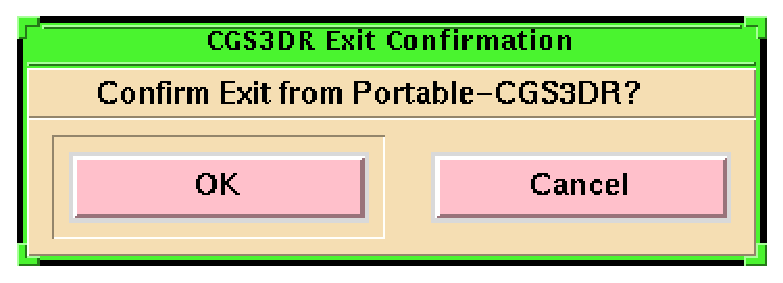
\includegraphics{sun206_fig1.ps}}}
  \end{picture}
  \caption{The Exit Confirmation Box} \label{sun206_fig1}
 \end{center}
\end{figure}

The {\sf Help} menu is shown in figure \ref{sun206_fig2}.
The {\sf Author(s)}, {\sf Tcl/tk Version} and {\sf Portable-CGS3DR Version} items all write an information
string to the text pane. The {\sf Portable-CGS3DR WWW Page} and {\sf CGS3 WWW Page}
items invoke {\em separate} incantations of {\sc netscape}.
\begin{figure}[htpb]
 \setlength{\unitlength}{1mm}
 \begin{center}
  \begin{picture}(160,60)
   \put(-1,0){\makebox(160,60){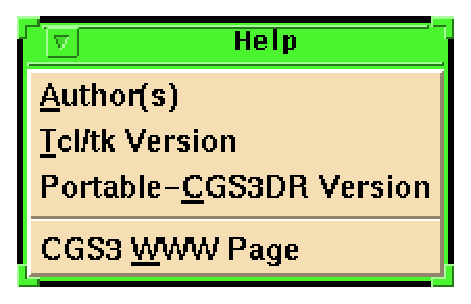
\includegraphics{sun206_fig2.ps}}}
  \end{picture}
  \caption{The Help Menu} \label{sun206_fig2}
 \end{center}
\end{figure}

The {\sf Options} menu is shown in figure \ref{sun206_fig3}.
\begin{figure}[htpb]
 \setlength{\unitlength}{1mm}
 \begin{center}
  \begin{picture}(160,60)
   \put(-1,0){\makebox(160,60){\includegraphics{sun206_fig3.ps}}}
  \end{picture}
  \caption{The Options Menu} \label{sun206_fig3}
 \end{center}
\end{figure}

The {\sf Set New Directory/Date} option returns the dialogue box shown in figure \ref{sun206_fig4} and is used
to re-initialise the software for another dataset without exiting the interface.
\begin{figure}[htpb]
 \setlength{\unitlength}{1mm}
 \begin{center}
  \begin{picture}(160,60)
   \put(-1,0){\makebox(160,60){\includegraphics{sun206_fig4.ps}}}
  \end{picture}
  \caption{The Set Directory/Date Option} \label{sun206_fig4}
 \end{center}
\end{figure}

The {\sf Clear Text Widget} option clears the text pane for the given task.

The {\sf Send Task an Action} returns the dialogue box shown in figure \ref{sun206_fig5} requesting an
action name to send to the selected task and is used for debugging.
\begin{figure}[htpb]
 \setlength{\unitlength}{1mm}
 \begin{center}
  \begin{picture}(160,100)
   \put(-1,0){\makebox(160,100){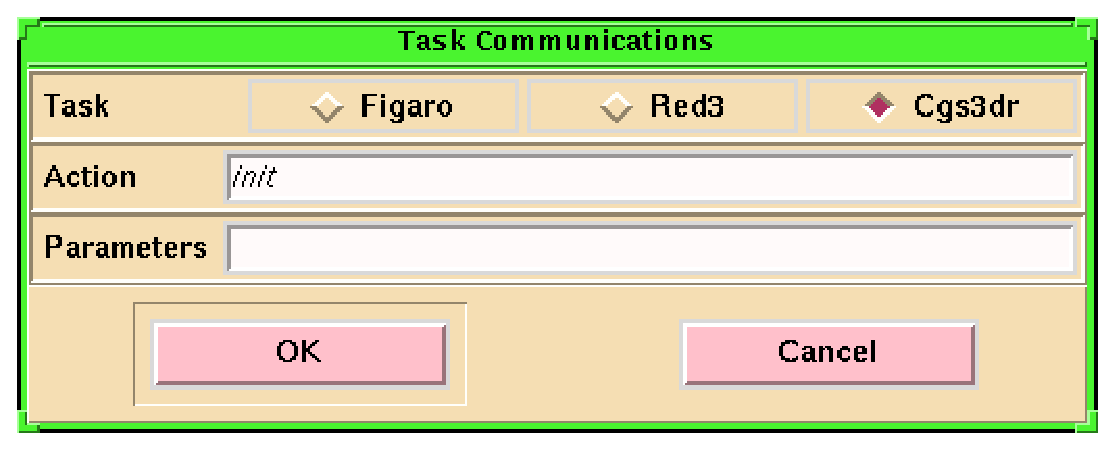
\includegraphics{sun206_fig5.ps}}}
  \end{picture}
  \caption{The Task Action Option} \label{sun206_fig5}
 \end{center}
\end{figure}

\subsection{The Text Pane}
The text pane is a large area which the tasks use to output their
messages of any type. It is not writeable by the user but may be
cleared from the {\sf Options} menu using {\sf Clear Text Widget}.

\subsection{The Widget Tree}
The widget tree is specific to each task. They are dealt with in separate chapters.

\section{Starting the Software}
The Portable-CGS3DR {\sc gui} can be started with two optional command line
parameters:

\begin{minipage}{120mm}
\begin{quote}
  \$1 is a data directory \hfill /\$\{home\}/ \\
  \$2 is a UT date \hfill /current UT-date/ \\
\end{quote}
\end{minipage}

To start the software, source the {\sc starlink} login and cshrc files and
use your local data directory. {\em E.g.:}

\begin{minipage}{120mm}
\begin{quote}
  \%  source \ \ /star/etc/login \\
  \%  source \ \ /star/etc/cshrc \\
  \%  cgs3dr\_tcl \ \ /scratch/pnd/19940811 \ \ 940811
\end{quote}
\end{minipage}

If any of the command line parameters are missing, a confirmation dialogue box
is created as shown in figure \ref{sun206_fig4}. Items labelled in {\em red} script within this box are those that
require confirmation.

Once started, as a background job, the window shown in figure \ref{sun206_fig6} will appear.
This has a red background to indicate `stop' whilst the tasks are loaded.
As each task becomes available, the appropriate traffic light will change to
green. When all three tasks are `go', the window disappears to be replaced by
2 full-size windows (cgs3dr and cgs3dr\_plot).
At this point, Portable-CGS3DR using {\sc tcladam} is
ready.
\begin{figure}[htpb]
 \setlength{\unitlength}{1mm}
 \begin{center}
  \begin{picture}(160,75)
   \put(-1,0){\makebox(160,75){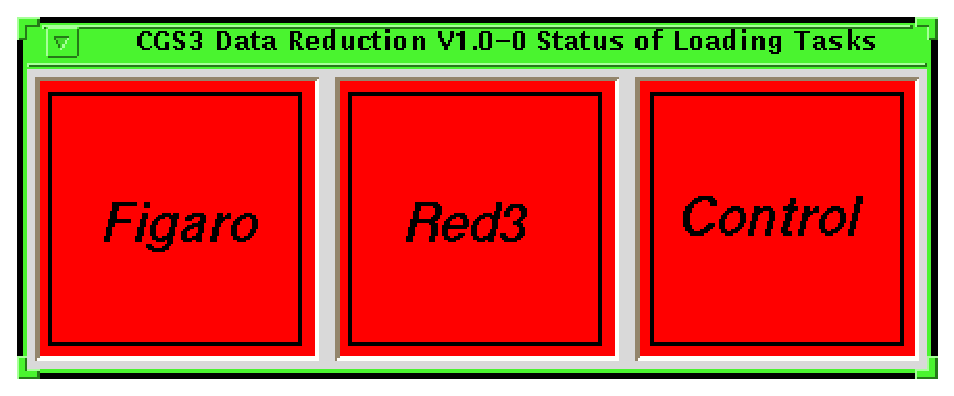
\includegraphics{sun206_fig6.ps}}}
  \end{picture}
  \caption{The Startup Box} \label{sun206_fig6}
 \end{center}
\end{figure}

\section{Common Problems Upon Startup}
\begin{description}
\item[] {\sf /star/bin/cgs3dr/tcl/cgs3dr\_tcl: Command not found.}

  The awish program has not been found.

  By default, awish is installed in /star/bin/awish and this is reflected
  in the first line of the file {\sc \$cgs3dr\_dir}/cgs3dr\_tcl:
  \begin{verbatim}
           #!/star/bin/awish -file
  \end{verbatim}
  If awish has been installed elsewhere, this line will need editing to reflect
  the correct location.

\item[] {\sf Invalid command name ``adamtask''.}

  The {\sc adam} extensions to tcl are not readable.

  The {\sc tcladam} software specifies a series of extensions to tcl that allow
  communications with the {\sc adam} messaging system and, hence, the tasks. These
  extensions are held in some directory in a file called adamtask.tcl (and others).
  The {\sc gui} startup file {\sc \$cgs3dr\_dir}/cgs3dr\_tcl has a line thus:
  \begin{verbatim}
           set tclAdamLib /star/lib/tk/adam
  \end{verbatim}
  This needs to reflect the location of your site's copy of the {\sc tcladam} software.

\item[] {\sf cgs3dr\_tcl aborting, failed creating task rendezvous file: File exists.}

  Task redezvous files were not deleted by previous shutdown.

  The task rendezvous files are located in the directory {\sc \$home}/adam and have the generic form
  {\sf xxxx}\_{\em task}\_{\sf yyyy} where {\sf xxxx} and {\sf yyyy} are unique numbers
  and {\em task} is one of the Portable-CGS3DR tasks (cgs3dr, red3 and figaro1).
  There are also files called cgs3dr\_tcl\_relay\_{\sf zzzz} and the like where {\sf zzzz}
  is another unique identifier. These are the task rendezvous files. If the software is,
  for example, aborted (using \% kill -9 {\em something}) rather than shutdown, these files may not be deleted.
  Subsequent attempts to run the software will fail until these rendezvous files are
  deleted. A list of current rendezvous files can be created thus:

  \begin{verbatim}
           % ls -l ~/adam | grep 'p---'
  \end{verbatim}

  Note that if you run the software more than once, some files are created with names such as
  `cgs3dr\_tcl \#2\_xxxx'. The quotes are deliberate as the filename contains a space character
  which is completely legal under Unix. Such files must be deleted properly.

\item[] {\sf Unable to allocate colour cells.}

  Software could not allocate enough colour cells.

  The number of colour cells is finite. Running too many (colour) applications (such as
  netscape, xmosaic etc) can exhaust the number of colour cells resulting in a failure
  to load the {\sc gui}. If this happens, you must delete some applications.
\end{description}

\chapter{The CGS3DR Interface}
\markboth{CGS3DR Interface}{\stardocname}
\section{The CGS3DR Interface}
The CGS3DR interface is shown in figure \ref{sun206_fig7}.
The interface is divided into two for controlling the CGS3DR and RED3 tasks.

The left hand side of the interface is for CGS3 task actions an each is invoked using
an action button. For the reduction actions, a run number must be specified in the
entry field. For the `Set Parameters' action the dialogue box shown in figure \ref{sun206_fig8}
is returned. The defaults button sets the defaults from the ADAM parameter system.

The right hand side of the interface controls actions in the RED3 monolith and are
invoked by {\em double-clicking} with the mouse on any item in the
listbox. Each item returns a dialogue box containing the parameters pertinent to that
tasks action. These are not shown.

\begin{figure}[htpb]
 \setlength{\unitlength}{1mm}
 \begin{center}
  \begin{picture}(160,160)
   \put(-1,0){\makebox(160,160){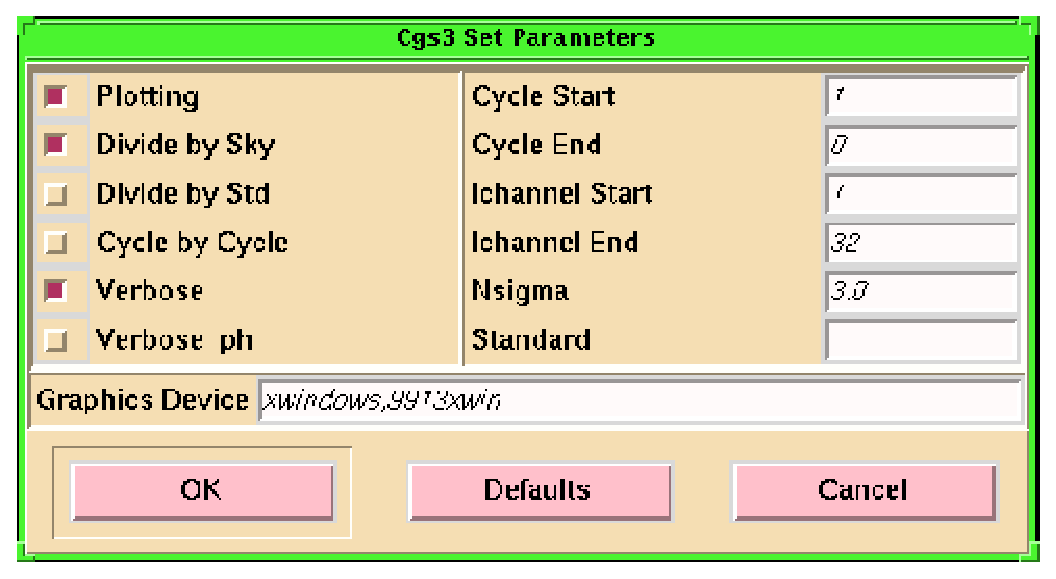
\includegraphics{sun206_fig8.ps}}}
  \end{picture}
  \caption{The Set Parameters Dialogue Box} \label{sun206_fig8}
 \end{center}
\end{figure}

\newpage
\begin{figure}[b]
 \setlength{\unitlength}{1mm}
 \begin{center}
  \begin{picture}(160,60)
   \put(-1,0){\makebox(160,60){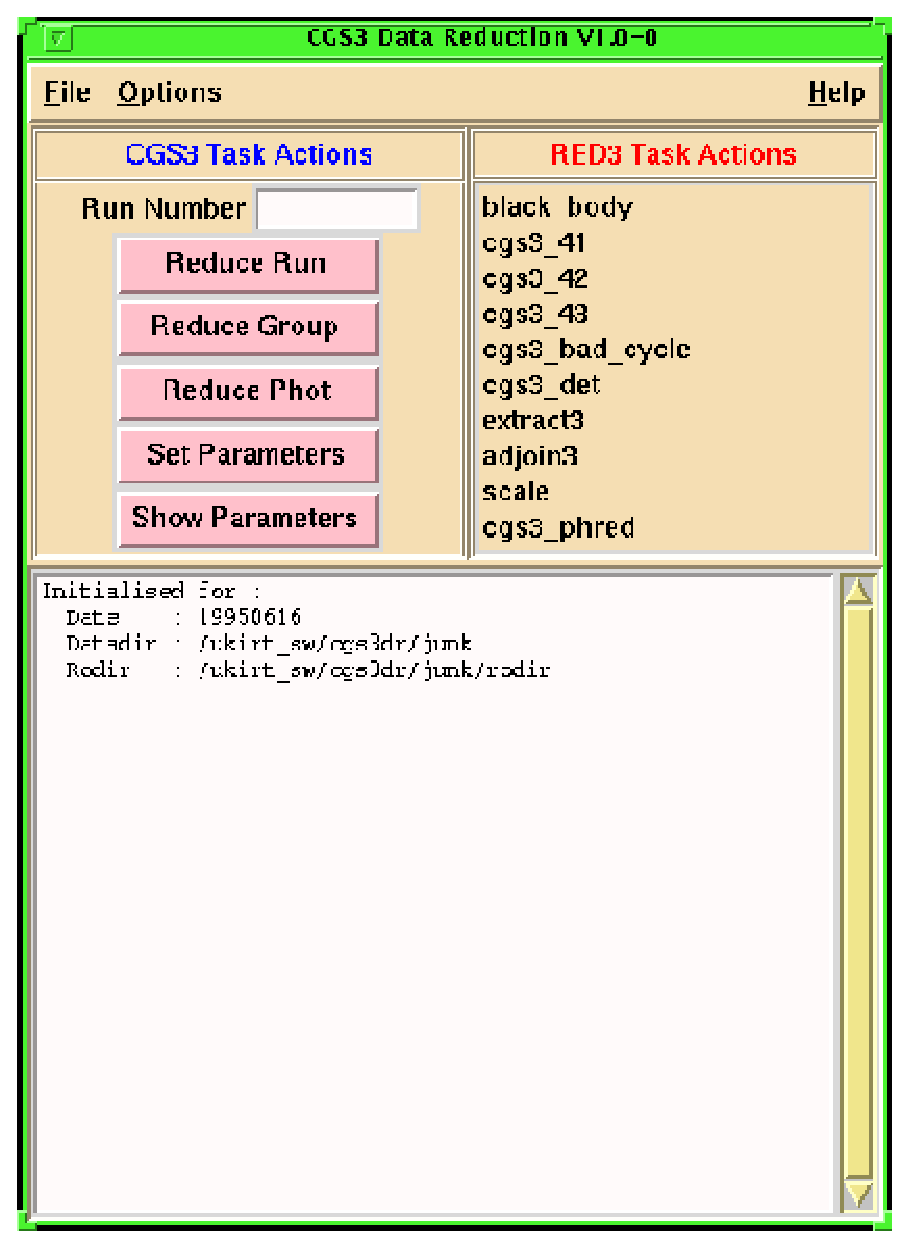
\includegraphics{sun206_fig7.ps}}}
  \end{picture}
  \caption{The CGS3DR Interface} \label{sun206_fig7}
 \end{center}
\end{figure}

\chapter{Miscellaneous}
\markboth{Miscellaneous}{\stardocname}
\section{May I run the {\sc gui} More Than Once?}
No, although this is being investigated.

\section{May I Run the Software in Batch?}
No. Unix does not recognize `batch' mode. The {\sc tcladam} interface, by default,
runs as a background job but the system is inherently interactive.

\section{Do I Still Need to Run the Kill Script?}
No. This was necessary under OSF/1 and an earlier version of ICL but no more. The
script has been retained, however, to start with a `clean' system when desired.

\section{How Do I Print Graphics?}
The {\sc gwm} widget is delivered with an action button labelled {\sf Print}. When
invoked, this returns a dialogue box tailoring the output to a variety of postscript
formats via an intermediate file. The file can be printed in the usual way.

\section{How Do I Check the Status of the Tasks?}
This is done on a task-by-task basis via the {\sf Options}
menu. Click on the item {\sf Send Task an Action} and input the action name `status'
into the data entry field. Then click on {\sf OK}.

\section{How Do I Start from Scratch?}
\label{restart}
If you encounter several problems and wish to revert to a known state, do the following:

\begin{quote}
  \% \ cgs3dr\_kill \\
  \% \ rm -f \ $\sim$/adam/* \\
\end{quote}

%%-----------------------------------------------------------------------------
%  References
\chapter*{References}
\markboth{References}{\stardocname}

\begin{description}
\item[] Shortridge, K. 1993, in  Astronomical Data Analysis Software
      and Systems II, A. S. P. Conf. Ser., Vol. 52, eds. R. J. Hanisch,
      R. J. V. Brissenden \& J. Barnes, p219-223.
\item[] Lawden, M. D., \& Hartley, K. F. 1992, SG/4, Starlink Project, CCL.
\item[] Ousterhout, J. K. 1994, `Tcl and the Tk Toolkit', ISBN 0--201--63337--X, Addison Wesley.
\item[] Terrett, D. L. 1995, SUN/186, Starlink Project, CCL.
\end{description}
\end{document}
